\documentclass[10pt,a4paper]{article}
\usepackage[latin1]{inputenc}
\usepackage{amsmath}
\usepackage{amsfonts}
\usepackage{amssymb}
\usepackage{graphicx}
\author{Emanuele Varriale}
\title{Notes on clique encoding networks}
\usepackage[backend=bibtex]{biblatex}
\bibliography{bibliography}
\begin{document}
	\maketitle
	\section{Introduction}
		The brain typically shows robust internal activity which is only modulated, but not driven, by sensory input, as the activity persists even in absence of such an input \cite{fiser_small_2004}. One could then wonder how does the internal dynamics relate to the sensory input and, in particular, how does meaning from the outside world get represented by network activity. 
		
		One possibility is to consider networks with transient state dynamics, i.e.\ networks whose activity consists of a series of attractor states, which are only transiently stable \cite{gros_semantic_2010}. Importantly, the attractor states themselves  are inherent to the network structure, and are not a product of external input. Such a network can be built as a collection of cliques, i.e.\ fully connected sub-networks. Connections  within cliques are only excitatory whereas among cliques they are mostly inhibitory, so that the network behaves in a multi-winner-take-all fashion. 
		
		The external input can then make use of pre-existing attractor states, acting as a bifurcation parameter, and confer semantic content to the network with a suitable learning rule that correlates input data to transient attractor dynamics. 
		
		We present a study on the internal transient state dynamics of networks with different architectures and, furthermore, we couple the network with an external input, from the bars problem, and analyse the resulting dynamics.
		
	\section{The network}
	\subsection{Architecture}
		Let's start by describing the possible network architectures for clique encoding. For simplicity we use undirected graph (i.e. symmetrical synapses) and neurons that have both excitatory and inhibitory synapses.
			
		One could build an Erd\"{o}s-Renyi kind of graph with excitatory connections and then complete the graph with inhibitory ones. This approach would lead to random cliques with an irregular autonomous dynamics, thus making even harder the search for a learning rule that couple cliques to sensory input.
			
		We have therefore worked with more regular networks which are described by the number of cliques $n_c$ and their size $s_c$. Each clique is a complete sub-graph with excitatory connections, and inhibitory connections exist only among different cliques. We worked with two kinds of networks which we named \emph{geometric} and \emph{rotating}, two examples are shown in Fig. \ref{fig:network}. 
		
		In the geometric arrangement each clique has two neurons that have an excitatory connection with another clique, while in the rotating arrangement every neuron of each clique has one such connection; but in both cases each clique can excite two other cliques. 
		
		The inhibitory connections either complete the graph, or are drawn with a probability P such that the average number of inhibitory synapses is equal to the number of excitatory ones.
		
		We will focus on the \emph{rotating} network.
		\begin{figure}
			\centering
			\includegraphics[width=0.45\linewidth]{../geometric/4x3net_r}
			\includegraphics[width=0.45\linewidth]{../rotating/4x3_sFalse.png}
			\caption{Left: a geometric network with $n_c = 3$ and $s_c = 3$. Right: a rotating network with $n_c = 3$ and $s_c = 4$.}
			\label{fig:network}
		\end{figure}
		
	\subsection{Weights}
		We choose the weights so that the input approximately lies in the range $[-1, \, 1]$. The activation function of neurons is a sigmoidal whose output is restricted to $[0, \, 1]$. To have the transient state dynamics we need high input for neurons belonging to the winning clique and negative input for those outside.
		We call the excitatory weights $w_{jk}$ and the inhibitory $z_{jk}$, $w_{jk}^{\text{inter}}$ are inter-clique excitatory connections.
		
		Let's consider then, respectively, neurons in the winning clique, and in the losing cliques only with negative inputs:
		\begin{equation}
			x_{\text{inp}} = \sum_{i=1}^{s_c - 1} w_{jk} y \approx \left(s_c -1 \right) \bar{w} \approx 1 \implies \bar{w} = \frac{1}{s_c - 1 }
		\end{equation}
		\begin{equation}
		x_{\text{inp}} = \sum_{i=1}^{s_c} z_{jk} y \approx s_c \bar{z} \approx -1 \implies \bar{z} = -\frac{1}{s_c}
		\end{equation}
		and for the inter-clique excitatory connections the input will be inevitably larger than the last case, for similarity with the above formulas, we choose 
		\begin{equation}
			w_{jk}^{\text{inter}} = \frac{1}{s_c} \implies x_{\text{inp}} \approx (s_c -1) \bar{z} +  \bar{w}^{\text{inter}} = -1 +\frac{2}{s_c}.
		\end{equation}
		We have neglected the small activities that would come from other neurons in the non-winning cliques.
		
	\section{Dynamics}
		By construction, if a clique is active it will inhibit every other clique and the state of the whole system will not change: it is an attractor. This is achieved by
		\begin{equation}
			\tau_x \dot{x}_j = -x_j + E_j + I_j, \quad E_j = \sum_{k} w_{jk} y_k, \quad I_j = \sum_k z_{jk} y_k
			\label{eq:neuron}
		\end{equation}
		\begin{equation}
			y_k = \sigma \left(x_k\right) = \frac{1}{1+\exp \left(a  \left(b - x_k \right)\right) }
			\label{eq:activation}
		\end{equation}
		with $\tau_x = 20 \ \text{ms}$,and $a$ and $b$ are, respectively the gain and the threshold of the sigmoidal.
		
		We now need a neuronal mechanism that causes a transient state dynamics by not allowing a high activity for a prolonged time. This was done in two ways: by a sliding threshold that limits the overall activity, and by limiting the pre-synaptic signal of each neuron.
		
		\subsection{Full depletion model}
		We employed a modified Tsodyks-Markram model which essentially describes the depletion of vesicles carrying neurotransmitters after sustained firing. Only the inhibitory synapses have this short-term plasticity so that a winning clique is not able, after a while, to inhibit every other neuron, so that a new winning clique will be established and so on. In practice the following was changed in Eq. \ref{eq:neuron} and \ref{eq:activation}:
		\begin{equation}
			I_j = \sum_k z_{jk} u_k \varphi_k y_k, \quad y_k = \frac{1}{1+\exp \left(- a x_k \right)}
		\end{equation}
		where $u$ controls the probability with which synaptic vesicles pop, and $\varphi$ models the number of available vesicles. In practice, there is an \emph{effective} pre-synaptic activity $\tilde{y}_k = u_k \varphi_k y_k$, as opposed to the ``somatic'' activity. These two additional variables have the following dynamics:
		\begin{equation}
			\dot{u}_j = \frac{U_y -u}{T_u}, \quad U_y = 1 + \left( U_\text{max} -1 \right) y_j, \quad U_\text{max} = 4
		\end{equation}
		\begin{equation}
		\dot{\varphi}_j = \frac{\varPhi_u - \varphi}{T_\varphi}, \quad \varPhi_u = 1- \frac{u y_j}{U_\text{max}},
		\end{equation}
		shown in the Fig. \ref{fig:full_depletion}. The pre-synaptic activity is completely shunted after sustained activity.
		
		\begin{figure}
			\centering
			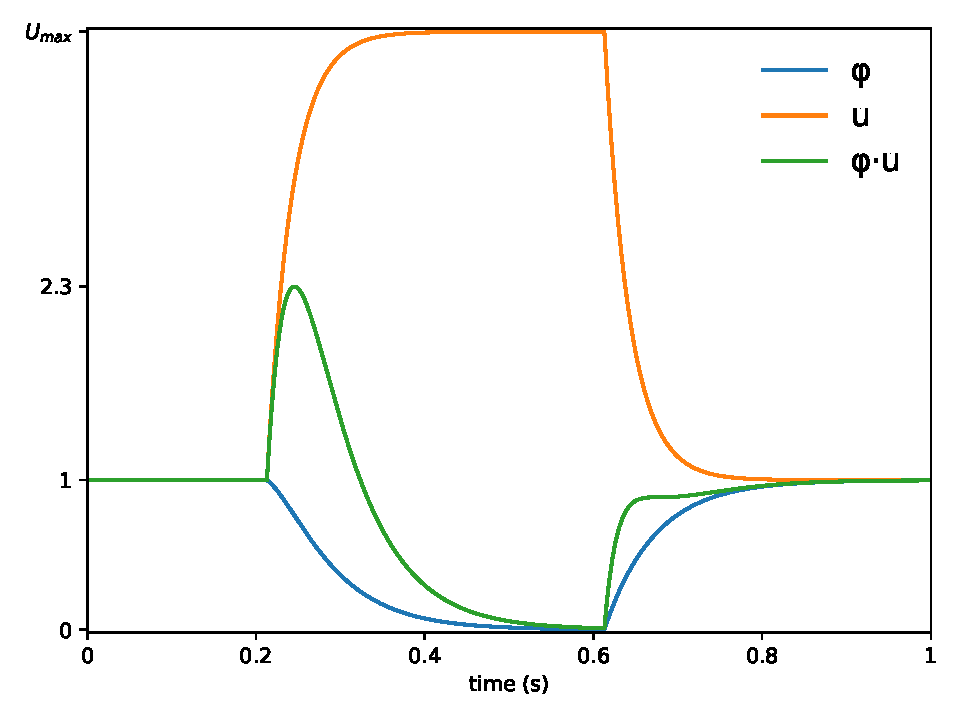
\includegraphics[width=0.7\linewidth]{./full_depletion}
			\caption{Short-term plasticity of a single neuron with high and low input. $T_\varphi=60 \ \text{ms}$, $T_u = 30 \ \text{ms}$}
			\label{fig:full_depletion}
		\end{figure}
		
		These rules can give rise to a transient state dynamics. As an example in a ring with 6 neurons, see Fig. \ref{fig:ring_activity} in which the activation function has a gain of $a=10$.
		
		\begin{figure}
			\centering

			\includegraphics[width=0.7\linewidth]{./ring_activity_g10}
			\includegraphics[width=0.5\linewidth]{./ring}
			\caption{}
			\label{fig:ring_activity}
		\end{figure}
		
		\paragraph{A few words on gains}
		It seems that an appropriately high value of the gain is needed in order to have transient state dynamics instead of a fixpoint, see Fig. \ref{fig:low_gain}, where the neuronal activities for gains $a=1,\ 5$ are shown. It seems that when the gain is too low, the activity does not get close to the extreme of $y = 1$ so the short-term plasticity does not kick in. This problem can be avoided with synaptic weights that are larger in absolute value. 
		
		In fact, consider that the intervals of $x$ in which the sigmoidal goes from $y=0.01$ to $y = 0.99$ for, respectively, gains $a = 1, \ 5, \ 10$ are $\left[-4.6,\ 4.6\right]$, $\left[-0.92,\ 0.92\right]$ and $\left[-0.46,\ 0.46\right]$, while the inputs are effectively restricted to $\left[-2.3,\ 1\right]$, the lower happening when the inhibitory synapses have their maximum efficacy.
		
		Since every neurons behaves the same, for $a=1$ it is possible to compute the steady state activity $y^* \approx 0.2625$ by solving numerically the self-consistent equation for $x_{\text{inp}}^*$:
		\begin{equation}
			x_{\text{inp}}^* = \left(2w_0 + 3 z_0 \varPhi_u^* U_y^* \right) y\left(x_{\text{inp}}^* \right)
		\end{equation}
		
		\begin{figure}
			\includegraphics[width=0.49\linewidth]{./ring_activity_g1}
			\includegraphics[width=0.49\linewidth]{./ring_activity_g5}
			\caption{If the gains are not large enough, the system rapidly goes to a fixpoint.}
			\label{fig:low_gain}
		\end{figure}
		
		\subsection{Learning rule}
		There can be another term that is added to the right hand side of the first equation in Eq. \ref{eq:neuron}, due to an external sensory signal:
		\begin{equation}
				\Delta E_j = \sum_l v_{jl} y_l, \quad v_{jl} > 0
		\end{equation}
		The input $\vec{y}$ comes from the bars problem and each $y_j$ can be either $0$ or $1$. 
		
		We are searching for a synaptic plasticity rule for the $v_{jl}$'s that works with the autonomous dynamics to ideally make each clique sensitive to a single bar.
		
		\paragraph{First rule $\dot{x}$}
		We first considered the following rule:

		\begin{gather}
		\tau_v \frac{d}{dt} v_{jl} = \dot{x}_j \left(\Delta E_j + I_j\right) v_{jl} c_j y_l\\
		c_j = \tanh{\left[10 \left(V_t - \Delta E_j \right)\right]}, \quad V_t = V^{\text{ina}} + y_j \left(V^{\text{act}} - V^{\text{ina}}\right) \\ 
		\tau_v = 200, \quad V^{\text{ina}} = 0.3, \quad V^{\text{act}} = 0.9,
		\end{gather}
		which does not lead to well defined receptive fields, as shown in Fig. \ref{fig:std_complete}. The response shape does not change much, but it lowers. This decrease is probably due to the normalization factor $c$, if removed the response increases.
		
		\begin{figure}[t]
			\centering
			\includegraphics[width=0.49\linewidth]{./8x4_g8_x}
			\includegraphics[width=0.49\linewidth]{./8x4_g8_xderivative}
			\label{fig:membrane_potential}
			\caption{On the left the membrane potential over time, on the right its derivative.}
		\end{figure}	
			
		\begin{figure}
			\centering
			\includegraphics[width=1\linewidth]{./complete_std2}
			\caption{Full lines show response after 6000 bar input, dashed lines show initial response. On the first row there is the input from the bars, on the second the receptive fields of the most responsive cliques, on the third every receptive field.}
			\label{fig:std_complete}
		\end{figure}
				
		The problems probably are:
			\begin{itemize}
				\item The membrane potential varies all of the time, see Fig. \ref{fig:membrane_potential}
				\item When a winning clique ``loses'', \emph{both} $\dot{x}_j$ and  $\left(\Delta E_j + I_j\right)$ are negative so that $v_{jl}$ is positive, modulo the normalization factor $c_j$
			\end{itemize}
		To address the first problem we replaced $\dot{x}_j$ with $\dot{y}_j$ by using
		\begin{equation}
		\frac{d}{dt}y(x) = a y (1-y) \dot{x}
		\end{equation}
		the result is basically the same, but the final response is even closer to the initial one.
		This also happens if instead of the term $\Delta E_j + I_j$ there $\sigma\left(\Delta E_j + I_j\right)$ which is non 0 only in the positive case.
		
		It seems that the normalization factor is doing most of the work, we have to think about that. A different approach could be to find a good rule for increasing the weights connecting the input neuron to the winning clique, and decreasing those connecting to different cliques, with some kind of competition of synapses belonging to the same input neuron.
		
		\newpage
		\paragraph{New network, simpler rule} One of the limitations of the above approach is that the network is effectively a \emph{ring} of cliques and external sensory input can only activate neighbouring cliques. So we have built a network in which every clique can activate any other.
		
		In this new network the autonomous dynamics is slower and cycles through only three cliques, even if there are more, see Fig \ref{fig:clique_net_activity}. It's not clear why previously active cliques receive a larger input, thus having a larger inhibitory effect, see Fig \ref{fig:clique_net_tsodyks}, and winning the competition. 
		
		\begin{figure}
			\centering
			\includegraphics[width=1\linewidth]{./clique_net_activity}
			\label{fig:clique_net_activity}
			\caption{With the new network only three cliques are visited}
		\end{figure}
		
		\begin{figure}
			\centering
			\includegraphics[width=1\linewidth]{./clique_net_tsodyks}
			\label{fig:clique_net_tsodyks}
			\caption{A clique wins when it gets larger input, thus larger inhibition due to the full depletion model}
		\end{figure}
		
		Despite this flaw, a simplified equation for $\dot{v}_{jl}$, with a learning term proportional to $\dot{y}_j$ and a slow decay term, namely:
		\begin{gather}
		\frac{d}{dt} v_{jl} = \dot{y}_j v_{jl} c_j y_l / \tau_v  - v_{jl} y_l / \tau_d\\
		c_j = \tanh{\left[10 \left(V_t - \Delta E_j \right)\right]}, \quad V_t = V^{\text{ina}} + y_j \left(V^{\text{act}} - V^{\text{ina}}\right) \\ 
		\tau_v = 1, \quad \tau_d = 600 000 \quad V^{\text{ina}} = 0.3, \quad V^{\text{act}} = 0.8,	
		\end{gather}
		after 400 bars input one gives the results shown in Fig. \ref{fig:comp_decay_ysens}, which are quite good.
		The very small time scale $\tau_v = 1$ is necessary because $\dot{y} \approx O\left(10^{-2}\right)$.
		
		\begin{figure}
			\centering
			\includegraphics[width=1\linewidth]{./comp_decay_ysens}
			\label{fig:comp_decay_ysens}
			\caption{}
		\end{figure}
		
		
		\begin{figure}
			\centering
			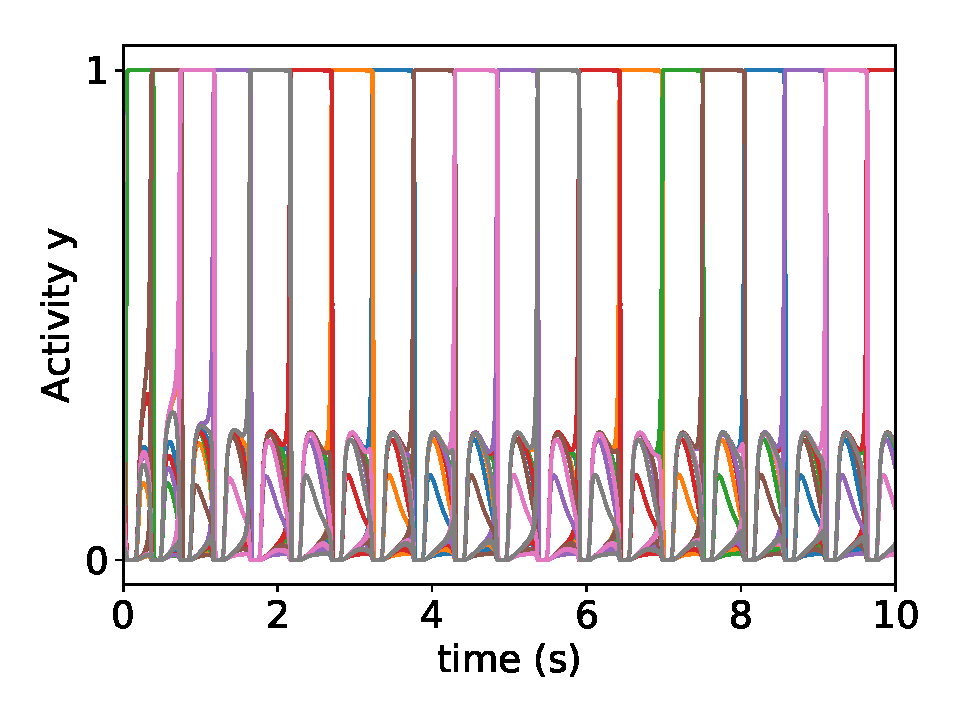
\includegraphics[width=0.8\linewidth]{./double_activity}
			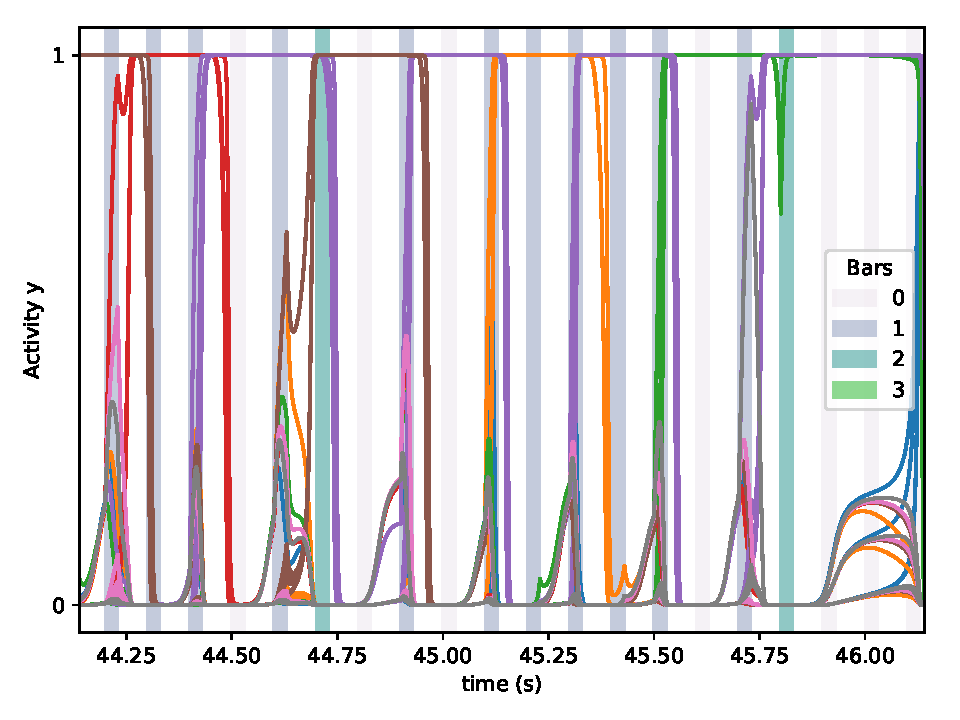
\includegraphics[width=0.8\linewidth]{./double_activity_legend}
			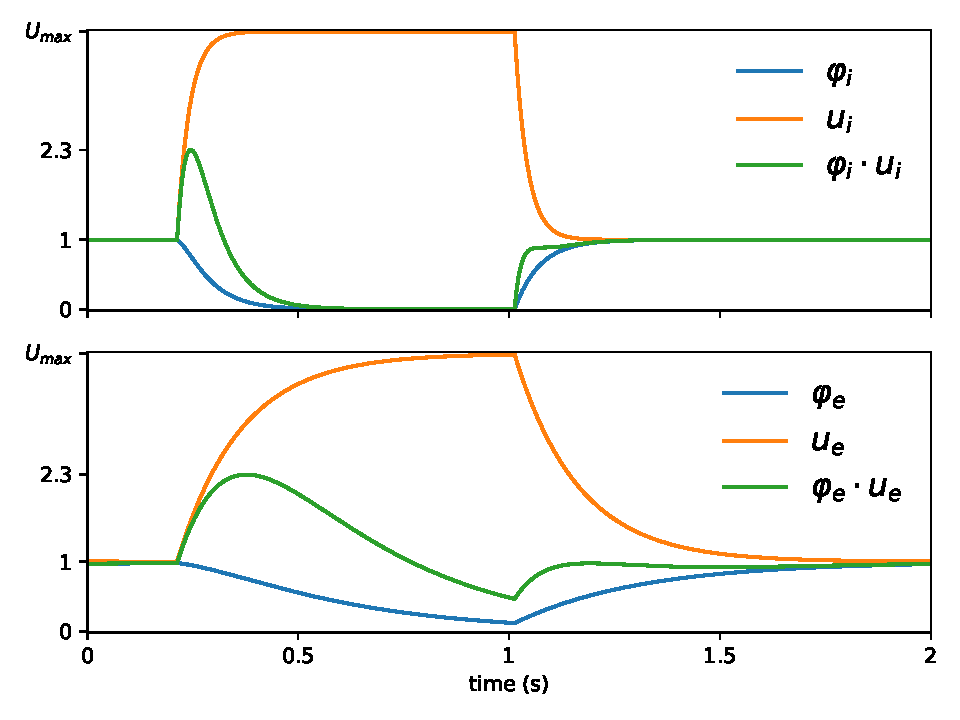
\includegraphics[width=0.8\linewidth]{./double_depletion}
		\end{figure}
				
		\begin{figure}
			\centering
			
			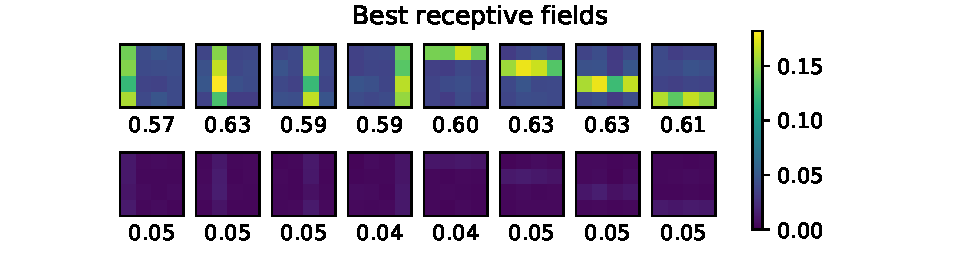
\includegraphics[width=1\linewidth]{./double_best_fields1}
			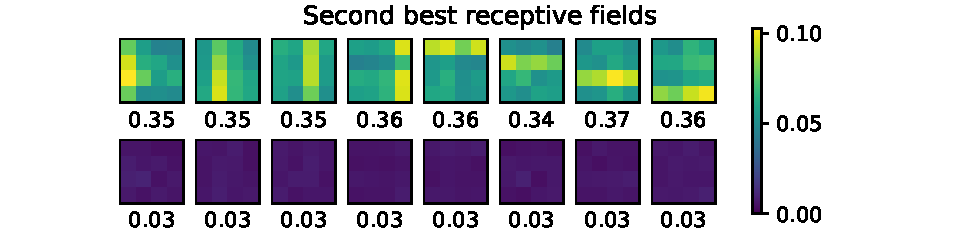
\includegraphics[width=1\linewidth]{./double_best_fields2}
			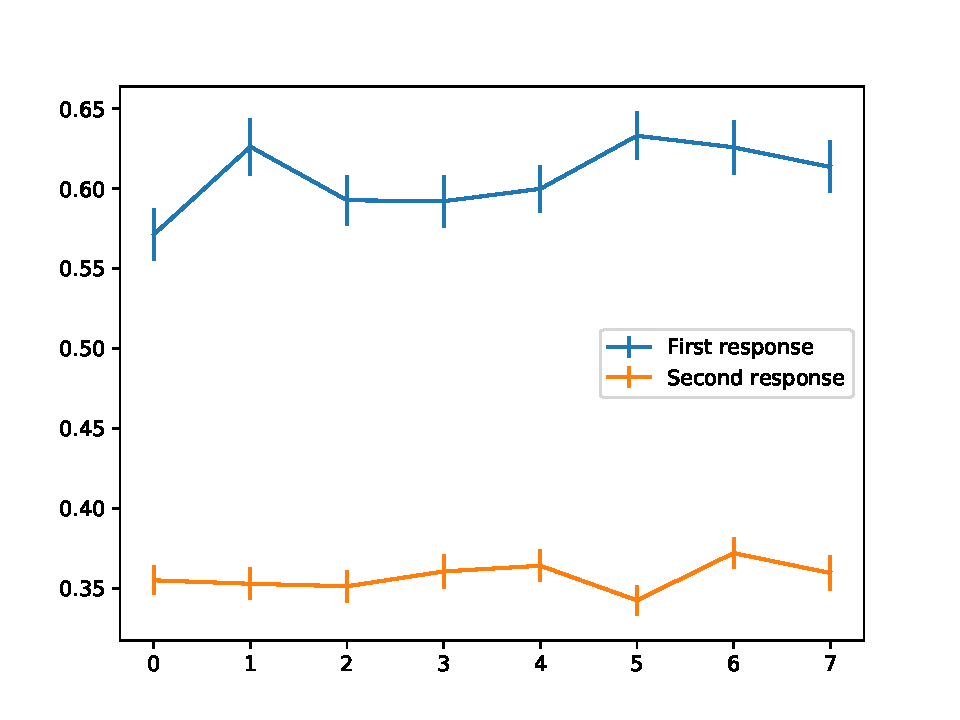
\includegraphics[width=1\linewidth]{./double_best_responses}
			\label{fig:comp_decay_ysens}
			\caption{}
		\end{figure}
		
		\newpage
		\printbibliography
\end{document}
